\section{Análisis tecnológico}

En esta sección se van a examinar algunas de las herramientas y conocimentos tecnológicos necesarios para el desarrollo posterior de la skill, de los que se ha podido generar una idea clara con el apoyo de la documentación oficial de Alexa \parencite{alexaDocs}.

\subsection{Justificación de la elección tecnológica}

En este apartado se justifica la elección de las herramientas y tecnologías utilizadas para el proyecto.

En cuanto a la elección del asistente de voz, se ha elegido \textbf{Alexa} por varios motivos, el principal porque el dispositivo disponible para el proyecto es un \textit{Amazon Echo Show 5}, y además se ha visto en las secciones \textit{2.3.2.} y \textit{2.3.3.} que es el asistente conversacional más extendido en la actualidad y tiene potencial para mejorar la calidad de vida de las personas mayores, entonces el producto final tendrá un mayor alcance.

Para el desarrollo de la habilidad, se ha decidido crear una skill alojada en Alexa (\textit{\textbf{Alexa-hosted skill}}) desde la consola de desarrolladores, por varios motivos: simplicidad en el despliegue, al delegar la labor de configuración y gestión de la escalabilidad de la función Lambda a Amazon, y por ofrecer un entorno de desarrollo integrado, con herramientas para facilitar la depuración y poder centrarse en la lógica más que en mantener la infraestructura. 

Para la skill alojada en Alexa, se ha decidido usar \textbf{Node.js} como entorno de ejecución en lugar de Python debido a que, a pesar de la simplicidad de este último, las características del primero en cuanto a rendimiento y escalabilidad lo hacen más apropiado en esta ocasión. Esto tiene su explicación en el modelo de Node.js, que trabaja con funciones asíncronas y eventos de entrada/salida no bloqueantes, lo que lo hace ideal para manejar varias tareas simultáneamente, sin tiempos de espera entre que cada una termina de finalizarse. Este aspecto es indispensable en los modelos de interacción por voz de las skill de las Alexa, que tienen requisitos en tiempo real. No solo eso, sino que también tras la investigación de recursos online y de ayuda relacionados con las skills de Alexa, se ha podido comprobar que Node.js contiene más material disponible.

Como mecanismo de almacenamiento de datos, se ha elegido la base de datos NoSQL de \textbf{DynamoDB}, puesto que al ser un servicio de AWS es fácil de integrar con la skill de Alexa, por no mencionar su escalabilidad y alto rendimiento en operaciones con un volumen cambiante de datos. Adicionalmente, para almacenar las imágenes necesarias para la interfaz del proyecto, se ha optado por \textbf{Amazon S3} por los mismos motivos que la base de datos seleccionada.

\subsection{Fundamentos de una skill}

Familiarizarse con los fundamentos de una skill implica comprender los conceptos clave usados en el contexto de una interacción entre una persona usuaria y Alexa, así como el funcionamiento general de la persistencia de datos dentro del código de la skill.

\subsubsection{Términos comunes en el desarrollo de skills}

Para comprender mejor la terminología en la documentación de este proyecto, se explican los conceptos siguientes:

\begin{itemize}
	\item \textit{\textbf{Intents}}: representan las intenciones de las personas usuarias, entendidas como las acciones llevadas a cabo con una finalidad, las cuales son llamadas a través determinadas frases. Por ejemplo, el intent \textit{guardarPartidaIntent} cumple con el objetivo de guardar el estado de la partida.
	\item \textit{\textbf{Utterances}}: son precisamente las frases de activación que se mencionaban antes. Explicado de otra forma, serían los comandos de voz que pueden utilizarse para invocar intents específicos, por lo que deben ser frases intuitivas y que difieran entre sí. Siguiendo el caso anterior, si se quiere llamar a \textit{guardarPartidaIntent}, las utterances podrían ser <<guarda mi partida>>, <<guárdame la partida>>, etc.
	\item \textit{\textbf{Handlers}}: son funciones encargadas de implementar la lógica de una skill. Están asociados a un intent para ejecutar el código que procese la respuesta esperada de dicho intent. Por ejemplo, el manejador \textit{guardarPartidaHandler}, que encapsula la lógica necesaria para el intent de ejemplo.
	\item \textit{\textbf{Slots}}: los intents pueden tener definidos slots de manera opcional. Se podrían describir como argumentos que Alexa captura de una determinada solicitud o respuesta de la persona usuaria, y que permiten guardar valores concretos para completar la lógica de los manejadores. Un ejemplo es si se tiene un intent, \textit{crearJugadoresIntent}, que cualquier usuario/a puede invocar diciendo <<Crea [tres] jugadores>>. Tres es capturado por el slot configurado para guardar el número de jugadores a crear.
\end{itemize}

\subsubsection{Memoria y persistencia de datos}

Entender cómo funciona la persistencia de datos en las skills es esencial para saber cómo abordar su desarrollo y garantizar que se mantiene un contexto adecuado durante toda la interacción con Alexa.

Se distinguen los dos mecanismos principales para la memoria de datos en skills que serán considerados para este proyecto: los atributos de sesión (\textit{session attributes}) y las bases de datos.

Los atributos de sesión, como da a entender el nombre, se ubican en el contexto de la sesión activa actual. Resultan útiles cuando se quiere mantener cierta información de un handler a otro, pero de manera temporal.

A continuación, se muestran los métodos básicos de consulta (o acceso) y modificación de un atributo de sesión, facilitados por la clase gestora de atributos que proporciona el SDK de Alexa (biblioteca específica de ASK, ver sección \textit{6.2.}).

\begin{figure}[H]
	\centering
	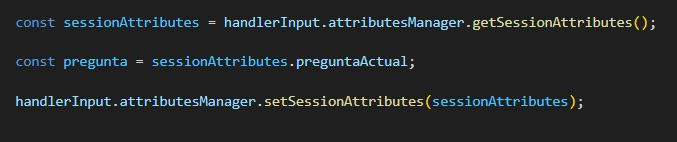
\includegraphics[width=0.93\textwidth]{imgs/sesion-atrib.jpg}
	\caption{Métodos básicos del gestor de atributos}
	\label{fig:sesion-atrib}
\end{figure}

Por otro lado, las bases de datos se diferencian en que sí permiten mantener información entre sesiones, de forma escalable y a largo plazo. Es la alternativa a tomar si se manejan estructuras de datos más complejas y/o necesarias en el contexto de futuras interacciones.

Las bases de dato pueden ser relacionales o no, aunque para las skills de Alexa es común optar por la opción NoSQL de \textit{DynamoDB}, puesto que es un servicio que ya viene integrado en AWS (ver sección \textit{6.3.}), adecuado gracias a su alta disponibilidad y buen rendimiento.

\subsection{Alexa Skills Kit (ASK)}

ASK es un conjunto de APIs y herramientas que facilitan la integración de nuevas habilidades en Alexa, permitiendo crear distintas clases de skills, desde personalizadas hasta otras específicas para vídeo, listas y hogar inteligente.

El tipo de skill que mejor se ajusta a los objetivos preestablecidos es la personalizada o \textit{Custom Skill}, pues esta permite más flexibilidad a los desarrolladores, permitiéndoles adaptarla a las necesidades de la aplicación a desarrollar.

Se puede importar ASK, a través del nombre de la biblioteca: \textit{ask-sdk-core}.

\subsection{AWS Serverless Platform}

Para el desarrollo de skills de Alexa, se puede optar o bien por la función Lambda de AWS, o bien por un servicio web distinto. La primera opción pertenece a un conjunto de herramientas de desarrollador y servicios en la nube de alto rendimiento que componen la Plataforma sin Servidor de AWS.

Se va a utilizar \textbf{AWS Lambda} para la creación de este juego digital, aprovechando así las múltiples funcionalidades y material de apoyo para encaminar el proceso de desarrollo. Además, al poder hacer uso de los otros servicios incluidos en esta plataforma (DynamoDB, Amazon S3, etc), se garantiza cierta centralización y absoluta compatibilidad entre ellos.

\subsection{Alexa Presentation Language (APL)}

La parte visual de la skill se gestiona mediante el lenguaje de presentación de Alexa (APL), a través del envío de documentos APL al dispositivo en forma de una directiva que se verá más adelante.

Un documento APL consiste en un fichero JSON que define la estructura y disposición de elementos a mostrar por la pantalla del dispositivo de Alexa.
A continuación se muestra un ejemplo básico de documento APL que imprime por pantalla una cadena de texto (\autoref{fig:apl-ejemplo}).

\begin{figure}[H]
	\centering
	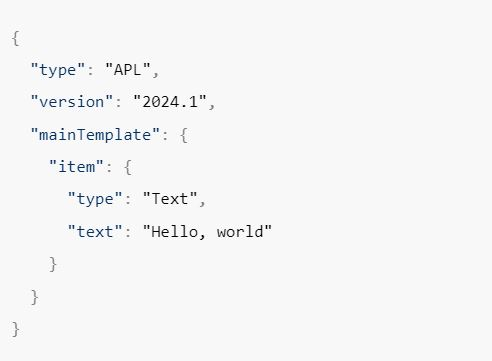
\includegraphics[width=0.6\textwidth]{imgs/apl-example.JPG}
	\caption{Ejemplo de documento APL básico (\href{https://developer.amazon.com/en-US/docs/alexa/alexa-presentation-language/apl-document.html}{Alexa Developer Docs})}
	\label{fig:apl-ejemplo}
\end{figure}

